\documentclass{standalone}
\usepackage{tikz}

\begin{document}

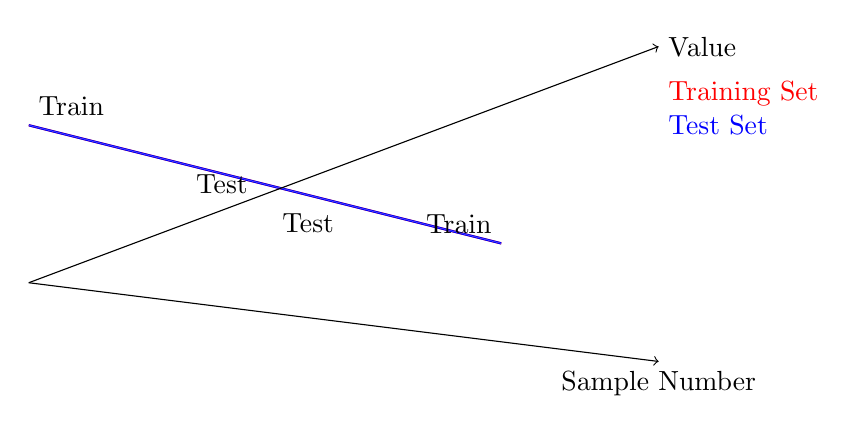
\begin{tikzpicture}[scale=2]
    % Define the points for the curve
    \coordinate (A) at (0,1);
    \coordinate (B) at (1,0.75);
    \coordinate (C) at (2,0.5);
    \coordinate (D) at (3,0.25);

    % Draw the curve
    \draw[thick, smooth, red] plot coordinates {(A) (B) (C) (D)};
    \draw[thick, smooth, blue] plot coordinates {(A) (B) (C) (D)};

    % Fill the area under the curve
    \fill[red!30] plot coordinates {(A) (B) (C) (D)} -- cycle;
    \fill[blue!30] plot coordinates {(A) (B) (C) (D)} -- cycle;

    % Add labels
    \node at (A) [above right] {Train};
    \node at (B) [below right] {Test};
    \node at (C) [below left] {Test};
    \node at (D) [above left] {Train};

    % Add legend
    \node at (4,1.2) [right] {\textcolor{red}{Training Set}};
    \node at (4,1) [right] {\textcolor{blue}{Test Set}};

    % Axis
    \draw[->] (0,0) -- (4,1.5) node[right] {Value};
    \draw[->] (0,0) -- (4,-0.5) node[below] {Sample Number};
\end{tikzpicture}

\end{document}